\documentclass[border=4pt]{standalone}
% Shared style for every diagram. Colour-blind-safe palette (Okabe-Ito).
\usepackage[T1]{fontenc}
\usepackage{helvet}
\renewcommand{\familydefault}{\sfdefault}
\usepackage{tikz}
\usetikzlibrary{arrows.meta,positioning,fit,backgrounds,calc,shapes.geometric,decorations.pathreplacing}
\definecolor{cblue}{HTML}{0072B2}
\definecolor{corange}{HTML}{E69F00}
\definecolor{cgreen}{HTML}{009E73}
\definecolor{cred}{HTML}{D55E00}
\definecolor{cpurple}{HTML}{CC79A7}
\definecolor{cgrey}{HTML}{6B7280}
\definecolor{csky}{HTML}{56B4E9}
\tikzset{
  >={Stealth[length=2.2mm]},
  box/.style={draw, rounded corners=3pt, align=center, minimum height=11mm, minimum width=22mm, font=\small, line width=0.7pt},
  real/.style={box, draw=cblue, fill=cblue!8},
  sim/.style={box, draw=corange, fill=corange!12},
  future/.style={box, draw=cgrey, dashed, fill=white},
  flow/.style={->, line width=0.8pt, draw=black!75},
  dflow/.style={->, line width=0.8pt, dashed, draw=cgrey},
  lbl/.style={font=\scriptsize, text=black!70},
  group/.style={draw=black!25, rounded corners=6pt, inner sep=6pt},
}

\begin{document}
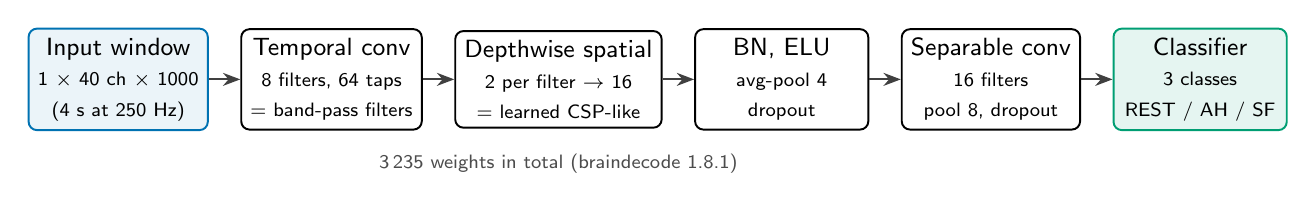
\begin{tikzpicture}[node distance=4mm, every node/.append style={minimum width=24mm, minimum height=15mm}]
  \node[real] (in) {Input window\\\scriptsize 1 $\times$ 40 ch $\times$ 1000\\\scriptsize (4 s at 250 Hz)};
  \node[box, right=of in] (t) {Temporal conv\\\scriptsize 8 filters, 64 taps\\\scriptsize = band-pass filters};
  \node[box, right=of t] (s) {Depthwise spatial\\\scriptsize 2 per filter $\to$ 16\\\scriptsize = learned CSP-like};
  \node[box, right=of s] (p1) {BN, ELU\\\scriptsize avg-pool 4\\\scriptsize dropout};
  \node[box, right=of p1] (sep) {Separable conv\\\scriptsize 16 filters\\\scriptsize pool 8, dropout};
  \node[box, draw=cgreen, fill=cgreen!10, right=of sep] (out) {Classifier\\\scriptsize 3 classes\\\scriptsize REST / AH / SF};
  \foreach \a/\b in {in/t, t/s, s/p1, p1/sep, sep/out} \draw[flow] (\a) -- (\b);
  \node[lbl, below=2mm of s, minimum height=0pt, minimum width=0pt] {3\,235 weights in total (braindecode 1.8.1)};
\end{tikzpicture}
\end{document}
